\newpage
\section{Vektorräume mit Skalarprudukt \texorpdfstring{$K=\mr$}{K=R}}

\subsection{Einführung}
	$\mr^2$

	\begin{tikzpicture}
		\draw (0,3) -- (0,0) -- (4,0);
		\draw [->] (0,0) -- (3.5,2.5);
		\draw (3.5,.1) -- (3.5,-.1) node[anchor = north]{$x_1$};
		\draw (.1,2.5) -- (-.1,2.5) node[anchor = east]{$x_2$};
		\draw [dotted] (3.5,0) -- (3.5,2.5) node[anchor = west]{$v\leftrightarrow\lrv{x_1\\x_2}$};
	\end{tikzpicture}

	\textbf{Länge} von $v$: $\lrabs{\lrabs{v}}=+\sqrt{x_1^2+x_2^2}$ (Pythagoras)

	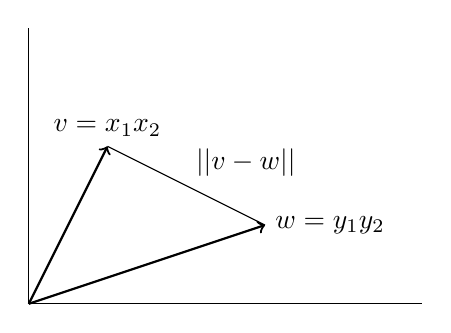
\begin{tikzpicture}
    \draw (0,0) -- (5,0);
    \draw (0,0) -- (0,3.5);
    \draw [->, thick] (0,0) -- (1,2) node [anchor=south] {$v=\lrv{x_1\\x_2}$};
    \draw [->, thick] (0,0) -- (3,1) node [anchor=west] {$w=\lrv{y_1\\y_2}$};
    \draw (3,1) -- node [anchor=south west] {$||v-w||$} (1,2);
  \end{tikzpicture}

	\textbf{Abstand} von $v,w$: $d\lrr{v,w}=\lrabs{\lrabs{v-w}}=+\sqrt{\lrr{x_1-y_1}^2+\lrr{x_2-y_2}^2}$

	\textbf{Winkel} (über Pythagoras)

  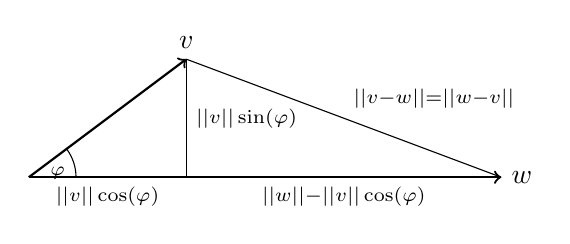
\begin{tikzpicture}
    \draw (2,0) -- node [anchor=west] {$\scriptstyle ||v||\sin(\varphi)$} (2,1.5);
    %\node [anchor=south] at (2,1.5) {$v$};
    %\node [anchor=west] at (6,0) {$w$};
    \path (2,0) -- node [anchor=north] {$\scriptstyle ||w||-||v||\cos(\varphi)$} (6,0);
    \path (0,0) -- node [anchor=north] {$\scriptstyle ||v||\cos(\varphi)$} (2,0);
    \draw [->, thick] (0,0) -- (2,1.5) node [anchor=south] (v) {$v$};
    \draw [->, thick] (0,0) -- (6,0) node [anchor=west] (w) {$w$};
    \draw (2,1.5) -- node [anchor=south west] {$\scriptstyle||v-w||=||w-v||$} (6,0);
    \draw (6mm,0mm) arc (0:36:6mm);
    \draw (.15,-.15) node [anchor=south west] {$\scriptstyle\varphi$};
  \end{tikzpicture}

	$\lrabs{\lrabs{v-w}}^2=\lrabs{\lrabs{v}}^2\sin^2\lrr{\varphi}+\lrr{\lrabs{\lrabs{w}}-\lrabs{\lrabs{w}}\cos\lrr{\varphi}}^2\\
	=\lrabs{\lrabs{v}}^2+\lrabs{\lrabs{w}}^2-2\lrabs{\lrabs{v}}\lrabs{\lrabs{w}}\cos\lrr{\varphi}$\\
	Mit Kosinussatz ($\sin^2(\varphi)+\cos^2(\varphi)=1$)

	$\lrabs{\lrabs{v-w}}^2=\lrr{x_1-y_1}^2+\lrr{x_2-y_2}^2=x_1^2+y_1^2+x_2^2+y_2^2-2x_1y_1-3x_2y_2$\\
	$\lrabs{\lrabs{v}}^2+\lrabs{\lrabs{w}}^2-2\lrr{x_1y_1+x_2y_2}$

	Es folgt:$\underbrace{x_1y_1+x_2y_2}_{\smt{Skalarprodukt}}=\lrabs{\lrabs{v}}\lrabs{\lrabs{w}}\cos\lrr{\varphi}$

\subsection{Definition}
	Seien $v,w\in\mr^n$ mit $v=\lrv{x_1\\\vdots\\x_n}, w=\lrv{y_1\\\vdots\\y_n}$\\
	Das \textbf{(Standard-) Skalarprodukt} von $v$ und $w$ ist\\
	$\lrr{v\mid w}=x_1y_1+x_2y_2+\dots+x_ny_n\;\;\in\mr$\\
	(Skalarprodukt von zwei Vektoren ergibt ereele Zahl)

	Es gilt
	\subExBegin{(1)}
		\item $\lrr{v\mid v}\geq 0$, $\lrr{v\mid v}=0\Leftrightarrow v=\sigma$\\
			(positiv definit)
		\item $\lrr{v\mid w}=\lrr{w\mid v}$ (symmetrisch)
		\item $\lrr{v\mid aw}=a\lrr{v\mid w}$\\
			$\lrr{v\mid w_1+w_2}=\lrr{v\mid w_1}+\lrr{v\mid w_2}$\\
			$\forall v,w,w_1,w_2\in\mr^n$ und $\forall a\in\mr$\\
			(Linearität im 2.Argument)
	\subExEnd
	Mit (2) und (3) folgt
	\subExBegin{(1)}
		\item[(4)] $\lrr{av\mid w}=a\lrr{v\mid w}$\\
			$\lrr{v_1+v_2\mid w}=\lrr{v_1\mid w}+\lrr{v_2\mid w}$\\
			$\forall v,v_1,v_2,w\in V, a\in\mr$\\
			Es gilt dann auch:\\
			$\lrr{\sigma\mid v}=\lrr{v\mid\sigma}=0$
	\subExEnd
	Dann heißt $V$ \textbf{Euklidischer} Vektorraum oder \textbf{Skalarproduktraum}.

\subsection{Beispiele}
	\subExBegin{a)}
		\item Das Standardskalarprodukt auf $\mr^n$ ist das Skalarprodukt im Sinne von 8.2
		\item $V$ ist $n$-dimensionaler $\mr$-Vektorraum.\\
			$\lrr{v_1,\dots,v_n}$ Basis von $V$.\\
			$v=\limsum{i=1}{n}a_iv_i$, $w=\limsum{i=1}{n}b_iv_i$\\
			$\lrr{v\mid w}:=\limsum{i=1}{n}a_ib_i$\\
			Skalarprodukt auf $V$.\\
			Standardskalarprodukt auf $\mr^n$ ist Spezialfall:\\
			Wähle Basis $\lrr{e_1,\dots,e_n}$
		\item $a,b\in\mr, a<b$\\
			$C\lra{a,b}=$ Vektorraum der stetigen Funktionen $\lra{a,b}\rightarrow\mr$\\
			$f,g\in C\lra{a,b}$:\\
			$\lrr{f\mid g}:=\limint{a}{b}f(x)g(x)\intd{x}\in\mr$\\
			Skalarprodukt auf $C\lra{a,b}$.\\
			\subExBegin{(1)}
				\item $\lrr{f\mid f}=\limint{a}{b}f^2(x)\intd{x}\geq 0$\\
					$f\neq 0: \lrr{f\mid f}>0$\\
					Dann $f^2>0$, also $\lrr{f\mid f}> 0$\\
					($f$ stetig nach MAthe 2)
			\subExEnd
	\subExEnd

\subsection{Satz - Cauchy-Schwarz'sche Ungleichung}
	$V$ Euklidischer Vektorraum.\\
	Dann $\forall v,w\in V: \lrr{v\mid w}^2\leq\lrr{v\mid v}\cdot\lrr{w\mid w}$\\
	Gleichheit $\Leftrightarrow v,w$ lin. abhängig

	\textbf{Beweis}

	Ist $w=\sigma$, so stimmt die Aussage des Satzes. Ist $w\neq 0$, so setze $aO\frac{\lrr{v\mid w}}{\lrr{w\mid w}}\in\mr$\\
	(Da $\lrr{w\mid w}> 0 (1)$)

	$0\ouset{\leq}{}{(1)}\lrr{v-aw\mid v-aw}\ouset{=}{}{(3)}\lrr{v-aw\mid v}-a\lrr{v-aw\mid w}$\\
	$\ouset{=}{}{(4)}\lrr{v\mid v}-a\lrr{w\mid v}-a\lrr{v\mid w}+a^2\lrr{w\mid w}$\\
	$\ouset{=}{}{(2)}\lrr{v\mid v}-2a\lrr{v\mid w}+a^2\lrr{w\mid w}$\\
	$\ouset{=}{}{\smt{Def. a}}\lrr{v\mid v}-\frac{2\lrr{v\mid w}^2}{\lrr{w\mid w}}+\frac{\lrr{v\mid w}^2}{\lrr{w\mid w}}$\\
	$=\lrr{v\mid v}-\frac{\lrr{v\mid w}^2}{\lrr{w\mid w}}$\\
	$\ouset{\Rightarrow}{}{\lrr{w\mid w}>0} 0\leq\lrr{v\mid v}\lrr{w\mid w}-\lrr{v\mid w}^2$\\
	Gleichheit $\Leftrightarrow\lrr{v-aw\mid v-aw}=0\ouset{\Leftrightarrow}{}{(1)}v=aw$, $v,w$ linear unabhängig.

\subsection{Definition}
	$V$ Euklidischer Vektorraum mit Skalarprodukt $\lrr{.\mid .}$
	\subExBegin{a)}
		\item Für $v\in V$ ist die \textbf{(Euklidische) Norm} von $v$ durch $\lrabs{\lrabs{v}}:=+\sqrt{\lrr{v\mid v}}$
		\item Für $v,w\in V$ ist der \textbf{Euklidscher Abstand} von $v$ und $w$ definiert durch\\
			$d\lrr{v,w}:=\lrabs{\lrabs{v-w}}$
	\subExEnd
	Damit lässt sich 8.4 schreiben als: $\lrabs{\lrr{v\mid w}}\leq\lrabs{\lrabs{v}}\cdot\lrabs{\lrabs{w}}$

\subsection{Beispiele}
	\subExBegin{a)}
		\item Standardskalarprodukt auf $\mr^n$:\\
			$v=\lrv{x_1\\\vdots\\x_n}, w=\lrv{y_1\\\vdots\\y_n}$\\
			$\lrabs{\lrabs{V}}=+\sqrt{x_1^2+\dots+x_n^2}$\\
			$d\lrr{v,w}=+\sqrt{\lrr{x_1-y_1}^2+\dots+\lrr{x_n-y_n}^2}$\\
			$n=2,3$ entspricht geometrischer Länge
		\item $V=C\lra{a,b}$\\
			$\lrr{f\mid g}=\limint{a}{b}f\lrr{x}g\lrr{x}\intd{x}, \lrabs{\lrabs{f}}+\sqrt{\limint{a}{b}f(x)^2\intd{x}}$
	\subExEnd

\subsection{Satz - Eigenschaften der Norm}
	$V$ Euklidscher Vektorraum mit Euklidscher Norm $\lrabs{\lrabs{.}}$\\
	Dann gilt $v,w\in V, a\in\mr$
	\subExBegin{(1)}
		\item $\lrabs{\lrabs{v}}\geq 0; \lrabs{\lrabs{v}}=0\Leftrightarrow v=\sigma$ (Definitheit)
		\item $\lrabs{\lrabs{av}}=\lrabs{a}\cdot\lrabs{\lrabs{v}}$ (absolute Homogenität)
		\item $\lrabs{\lrabs{v+w}}\leq\lrabs{\lrabs{v}}+\lrabs{\lrabs{w}}$ (Dreiecksungleichung)

			$\mr^2$
			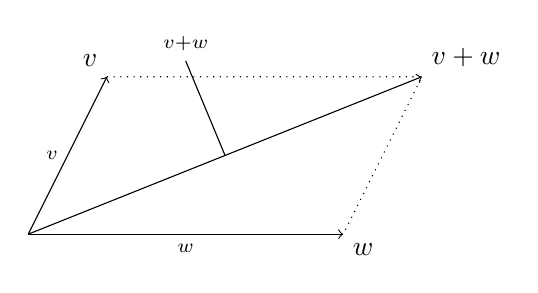
\begin{tikzpicture}
				\draw [->] (0,0) -- (2,0) node[anchor= north]{$\scriptstyle \lrabs{\lrabs{w}}$} -- (4,0) node[anchor= north west]{$w$};
				\draw [->] (0,0) -- (0.5,1) node[anchor= east]{$\scriptstyle \lrabs{\lrabs{v}}$} -- (1,2) node[anchor= south east]{$v$};
				\draw [->] (0,0) -- (5,2) node[anchor= south west]{$v+w$};
				\draw [dotted] (1,2) -- (5,2) -- (4,0);
				\draw (2.5,1) -- (2,2.2) node[anchor= south]{$\scriptstyle \lrabs{\lrabs{v+w}}$};
			\end{tikzpicture}
		\item $\lrabs{\lrabs{v+w}}^2=\lrabs{\lrabs{v}}^2+\lrabs{\lrabs{w}}^2+2\lrr{v\mid w}$
		\item $\lrabs{\lrabs{v+w}}^2+\lrabs{\lrabs{v-w}}^2=2\lrr{\lrabs{\lrabs{v}}^2+\lrabs{\lrabs{w}}^2}$ (Parallelogrammgleichung)

			$\mr^2$
			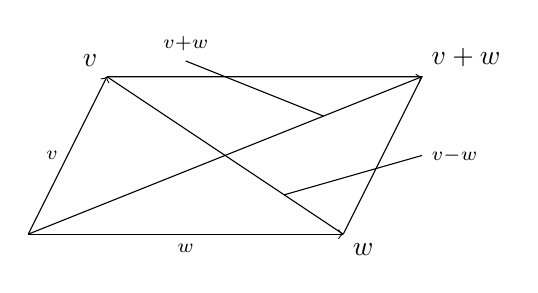
\begin{tikzpicture}
				\draw [->] (0,0) -- (2,0) node[anchor= north]{$\scriptstyle \lrabs{\lrabs{w}}$} -- (4,0) node[anchor= north west]{$w$};
				\draw [->] (0,0) -- (0.5,1) node[anchor= east]{$\scriptstyle \lrabs{\lrabs{v}}$} -- (1,2) node[anchor= south east]{$v$};
				\draw (1,2) -- (5,2) -- (4,0);
				\draw (3.75,1.5) -- (2,2.2) node[anchor= south]{$\scriptstyle \lrabs{\lrabs{v+w}}$};
				\draw [->] (0,0) -- (5,2) node[anchor= south west]{$v+w$};
				\draw (1,2) -- (4,0);
				\draw (3.25,0.5) -- (5,1) node[anchor=west]{$\scriptstyle \lrabs{\lrabs{v-w}}$};
			\end{tikzpicture}
	\subExEnd
	\textbf{Beweis}

		(1),(2) sind klar.
		(3),(4):\\
		$\lrabs{\lrabs{v+w}}^2=\lrabs{v+w\mid v+w}=\lrr{v\mid v}+\lrr{w\mid w}+2\lrr{v\mid w}\leftarrow (4)$\\
		$\ouset{\leq}{}{\smt{8.4}}\lrr{v\mid v}+\lrr{w\mid w}+2\sqrt{\lrr{v\mid v}\lrr{w\mid w}}$\\
		$=\lrr{\sqrt{\lrr{v\mid v}}+\sqrt{\lrr{w\mid w}}}^2=\lrr{\lrabs{\lrabs{v}}+\lrabs{\lrabs{w}}}^2$\\
		(5) folgt aus (4)

\subsection{Bemerkung}
	Für $\mr$-Vektorräume nennt man jede Funktion $\lrabs{\lrabs{.}}:V\rightarrow\mr_{\geq 0}$ mit Eigenschaften (1),(2),(3) aus 8.7 eine \textbf{Norm}.\\
	Dann gibt es auch andere Normen als solche, die über Skalarprodukte definiert werden.\\
	Zum Beispiel $\mr^n, \lrabs{\lrabs{\lrv{x_1\\\vdots\\x_n}}}_{\smt{max}}:=\mbox{max}\lrc{\lrabs{x_i}:i=1,\dots,n}$

\subsection{Definition}
	\subExBegin{a)}
		\item C-S-Ungleichung 8.4. mit $v\neq\sigma, w\neq\sigma$:\\
			$\frac{\lrabs{\lrr{v\mid w}}}{\lrabs{\lrabs{v}}\lrabs{\lrabs{w}}}\leq 1$\\
			Das heist $-1\leq\frac{\lrr{v\mid w}}{\lrabs{\lrabs{v}}\lrabs{\lrabs{w}}}\leq 1$\\
			Daher gibt es geunau ein $\varphi\in\lra{0,\pi}$ mit $\frac{\lrr{v\mid w}}{\lrabs{\lrabs{v}}\lrabs{\lrabs{w}}}=\cos\lrr{\varphi}$\\
			($\mr^2$: Standarskalarprodukt: $\varphi=$ Winkel zwischen $v,2$)\\
			$\varphi$ heißt der \textbf{Winkel} zwischen $v$ und $w$ $\lrr{0\leq\varphi\leq\pi}$
		\item $v,w$ heißen \textbf{orthogonal} (senkrecht), falls $\lrr{v\mid w}=0$\\
			(das heißt Winkel zwischen $v$ und $w$ ist $\frac{\pi}{2}(\hat{=}90^\circ$\\
			$\sigma$ ist orthogonal zu allen Vektoren. $v \perp w$
		\item $M\mpo V$, so $M^\perp=\lrc{w\in V:\lrr{v\mid w}=0\forall v\in M}$\\
			\textbf{Orthogonalraum} zu $M$.

			\textbf{Beispiel} $\mr^2$ Standardskalarprodukt.\\
				$M=\lrc{\lrv{1\\2}}$\\
				$\lrr{\lrv{x\\y}\mid\lrv{1\\2}}=0$\\
				$x+2y=0\Leftrightarrow x=-2y$\\
				$\Rightarrow M^\perp=\lrc{\lrv{-2y\\y}: y\in\mr}=\lrg{\lrv{2\\-1}}_\mr$
	\subExEnd
